% !TEX root = _main.tex

%\title{持続音系楽器のための演奏表現付け支援システムの開発}
%\author{32145004　浅野　桐子}{ASANO Toko}{FUKU}[]


% ==========================================
% ここから本文．あとは各自で
% ==========================================

%1
\section{はじめに}

音楽における演奏は，聴き手に豊かな演奏を伝えることが求められる．そのために，楽譜上に記載された音符や強弱を正確に再現するだけでなく，演奏者自身が楽曲を解釈し，強弱やテンポの変化を施す作業が必要となる．複数のパートが存在する楽曲であれば，各パートに異なる演奏表現が必要となるため，その難しさはさらに高まる．旋律が複雑に絡み合う構成の楽曲では，演奏者が瞬間的に演奏表現の付与を行うことは容易ではない．

そこで本研究では，楽曲音源に演奏表現を挿入できるシステムの開発を行った．特に，ロングトーンにおける強弱変化や音符ごとの音量制御に焦点を当てている． 次章では，演奏表情付けのアプローチに関する先行研究を示し，本システムの設計に関して参考とした理論や技術について議論する．



%2
\section{先行研究}
\subsection{保科理論}
保科理論\cite{Hoshina98}とは楽譜上の音符の配列を力学的なエネルギーに例え，楽曲分析・演奏解釈を行っているものである．本研究では，フレーズや重心の考えを取り入れシステムの構築を行った．以下は参考箇所をまとめたものである．

\subsubsection{楽譜から読み解く音楽構造}
保科理論で提唱されている音楽構造（\figref{fig:hoshina}）は，楽譜上に書かれた音符の配列を階層構造化することにより，楽曲の盛り上がりが明確化される考え方である．
音楽経験者であれば，「ここの部分は山を描くような強弱表現で」といった非常に抽象的な指示をされることがある．音楽構造が明確になることにより，指導者から奏者への伝達が円滑に進むだけでなく，音楽初心者にも理解しやすい考え方となっている．
以下の３点は音楽構造を構成する要素である．


\begin{description}
	\item[(1)  グループ]
	      グループとは，複数音を一つのまとまりとみなしたもののことを指している．作曲家が楽譜上で提示した音符の並びから，演奏者が楽曲分析しながらグルーピングすることにより，音楽的意味を持たせる．
	\item[(2) 重心]
	      重心はグループの中に１つ存在しており，グループ内で最もエネルギーが集中する音符のことを指している．重心は演奏表現の核となるものであり，エネルギーの増幅・減衰を設計する基準点となる．
	      重心を決定づける要因は，音符の並びや和声，拍節，アーティキュレーションなどといった音楽的な観点から決定していく．
	\item[(3) フレーズ]
	      フレーズは，複数のグループによって構築される音楽表現の基本単位である．そのため，フレーズの中には複数の重心が含まれるが，いずれかがフレーズ全体の最重心として機能する場合が多い．
	      一見，グループとフレーズは似ているようにも思うが，文法に例えるとグループが「単語」，フレーズは複数の単語が集まってできた「文章」といったような感覚の違いがある．

\end{description}

\begin{figure}
	\centering
	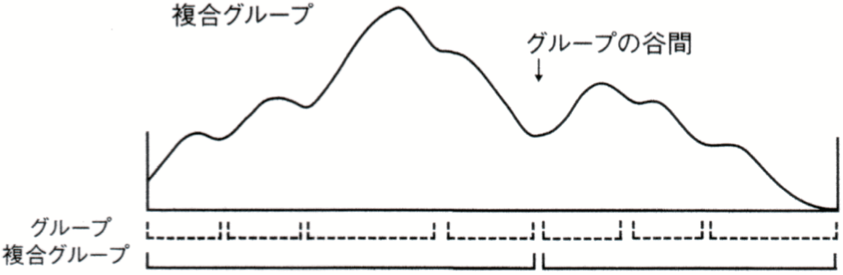
\includegraphics[width=\hsize]{fig/hoshina_phrasing.png}
	\caption{保科理論におけるフレーズの構造（文献\cite{Hoshina98}より抜粋）}
	\label{fig:hoshina}
\end{figure}
\subsubsection{楽曲の分析について}
保科理論における楽曲分析とは，演奏表現の基盤を形成する作業である．一般的に，演奏者は，楽譜上に書かれた情報から音楽的な要素を正確に読み取り演奏するという，概念的な作業として行われる．しかし，保科理論ではそういった作業にとどまらず，フレーズや重心の設定といった模式的な演奏解釈の作業を含め，楽曲分析としている．
また，重要な特徴として，解釈が一通りではないことが挙げられる．演奏者によって楽曲解釈の結果が異なることが充分に想定できる．分析結果が多様であっても，共通の原則に基づいていれば，それぞれが正当性を持つものとして受け入れられる．


\subsection{Mixtract:演奏表現のデザイン環境}
Mixtract\cite{mixtract}はフレーズ構造を基盤とした演奏表現をデザインするためのシステムである．ユーザが楽曲のフレーズ構造を設定し，その構造をもとに，テンポ，強弱，アーティキュレーションといった演奏表現が付与できる．またそのような機能に加え，認知的音楽理論であるGTTM\cite{gttm83}を応用し，演奏設計の自動補完も可能になっている．

ユーザの手順は，MusicXMLのインポート機能を利用し，楽譜情報を入力する．次にフレーズ構造の指定を行い，フレーズに対して表情カーブを決定する．表情カーブはテンポ，ダイナミクス，アーティキュレーションについての設定が可能である．

また，Mixtractは，ユーザ主導の演奏デザインを可能にすると同時に，認知的音楽理論や保科理論の応用により，フレーズ構造解析や表情カーブの設計を効率化している．以下はその機能についての概要をまとめたものである．

\subsubsection{フレーズ解析支援}
Mixtractでは，フレーズ構造解析支援として，ユーザが部分的に指定したフレーズをもとに，未指定部分のフレーズをGTTMの技術を応用し、解析する機能を備えている．そのため，フレーズの決定において，ユーザの負担が少ないフレーズ構造解析が可能になっている．
\subsubsection{フレーズ中の頂点推定}
保科理論に基づき，フレーズ内での頂点を推定し，演奏表現の設計を支援する．Mixtractでは，各音符のエネルギー値を表示し，音量やテンポなどの表現要素に変換する機能を提供している．また，保科理論では「重心」として定義されている．

\section{ロングトーンを考慮した演奏表現}
保科理論では奏者が感覚的に行っていた表現を視覚化する技術であることが確認できた．
また，Mixtractは，保科理論を基本的な設計思想に置き，ユーザが楽曲のフレーズ構造を効率的に設定できるデザイン環境を提供している．

本研究の設計思想も，基本的にはMixtractを踏襲したものである．
しかし，Mixtractをはじめとする従来の演奏表情付け研究では，鍵盤楽器でのMIDI表現を中心に開発されてきた．本章では保科理論の基本概念を再検討するとともに，管楽器における柔軟な演奏表現の可能性を踏まえた新たな視点を示唆する．
\subsection{ロングトーン表現の理論的基盤}
保科理論では，フレーズの中で音楽的な盛り上がりの重心を定義することで，楽曲の構造と表現を深く分析する手法を提供している．そのため，フレーズ単位での音量変化となっており，ロングトーンの観点では次の２点が定式化されている．

\begin{enumerate}
	\item フレーズの終了地点に向かっている音符に対しては，音量が減衰するものとされている
	\item 重心は音符の初期位置に定める
\end{enumerate}
これらの原則は，演奏する楽器の種類や音楽ジャンルに依存せず，普遍的に適用可能なものとして設計されている．このような表現方法が合理的かつ自然とみられることが多い．

鍵盤楽器の音は構造上，長時間音を持続させようとしても音量が減衰する性質を持っている．一方で，管楽器では，音量を持続させるだけでなく途中で音量を増加させるクレッシェンドのような表現も可能であり，これらの演奏特性は保科理論では十分に説明されていない．Mixtractにおいても，保科理論に準拠して設計されているため，ロングトーンに対しての仕様はない状態である．

よって，保科理論は，鍵盤楽器の特性に適している設計であることが明確化された．そこで本研究では異なる特定の楽器の柔軟性を取り込む余地があると考えた．次節では管楽器の特有の柔軟な強弱表現の可能性について詳しく検討する．
\subsection{管楽器におけるロングトーン表現の特性}
管楽器は，演奏方法において，鍵盤楽器とは大きく異なる特性を持つ．この特性は，特にロングトーン表現において顕著であり，管楽器独自の演奏表現であると考えられる．

鍵盤楽器と比較して，管楽器においては3.1節の２点とは異なる演奏が考えられる．

鍵盤楽器のロングトーンは，音量が減衰していくため，フレーズの重心が音符の先頭に置かれるという保科理論の原則が自然に適用される．

一方，管楽器は息でコントロールが可能なため，奏者の息が持続する限り，ロングトーンの途中の音量変化は自在である．そのため，管楽器であれば，ロングトーンの途中に重心を置き，音量が盛り上がる場合も大いに考えられる．
\begin{figure}[tb]
	\centering
	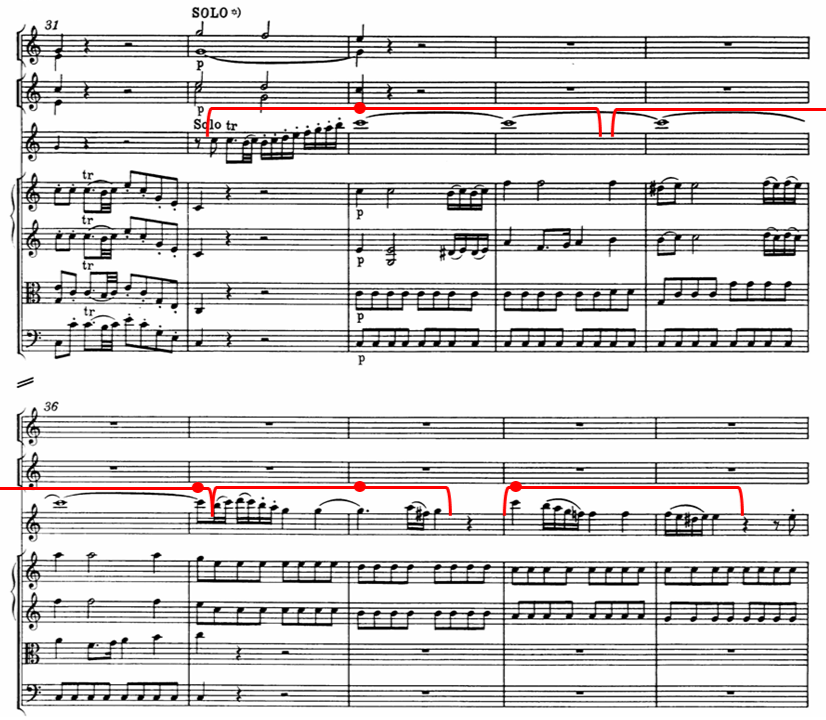
\includegraphics[width=\hsize]{fig/fig1-oboe.png}
	\caption{モーツァルト作曲「オーボエ協奏曲 ハ長調 K.314/271k」より，オーボエソロの長いフレーズ表現}
	\label{fig:oboe}
\end{figure}
\subsubsection{事例：オーボエ協奏曲}
ロングトーンの中間でフレーズの重心が考えられる例として，モーツァルト作曲のオーボエ協奏曲\cite{oboe}を挙げる．この楽曲は，オーボエと管弦楽のための協奏曲である上に，オーボエ協奏曲の中でもとりわけ知名度が高く，音大の入試やオーケストラの入団試験の際にも必ずといっていいほど演奏される楽曲となっている．

ロングトーンでの表現が明確に聞き取れるのが，オーボエソロが始まる冒頭部分で４小節間にもまたぐ長いロングトーンである．オーボエソロパートの楽譜では，強弱記号の指示は書かれていない．

オーボエ奏者の大多数の演奏を視覚化したものを\figref{fig:oboe}に示す．32小節目から演奏をはじめ，33小節目の音に向けてスケールを上ったのち，33小節～34小節の区間は他の管弦楽器に合わせ，音量を減衰すさせる．34小節の半ばあたりからフレーズが再度始まり，徐々にクレッシェンドしていく．そして，36小節目付近に差し掛かったあたりで，37小節目に向けて強くクレッシェンドする．図では，枠で囲ってあるのがフレーズ，丸で印をつけた位置をフレーズ内の重心としている．

特に，34～37小節の流れは鍵盤楽器には演奏できない強弱のコントロールである．

従って，管楽器ではロングトーン中でのクレッシェンドが頻繁に演奏される．



\subsection{ロングトーン表現の新たな視点}
管楽器におけるロングトーン表現は，従来の鍵盤楽器中心の理論では十分に説明できないことが明らかとなった．そのため，管楽器の特性を考慮する場合，別のアプローチが必要であると判断した．Mixtractでは指定したフレーズに対して，音が持つVelocityを操作することにより強弱表現を行っていた．しかし，管楽器の場合，3.2節のように必ずしも音の出だしに頂点が来るとは限らない．Velocityで操作を行うと，音が持続している最中に頂点を持ってくることは不可能であった．

そこで，Velocityではなく，Control Change（以下：CC）というパラメータで制御することにより，ロングトーンの途中でも強弱表現を行う手段を提案する．また，CC挿入時に用いる単位として「分解能」\cite{Tick}という単位を使用する．以下は，Velocity，Expressionそして分解能について説明する．
\subsubsection{Velocityについて}
VelocityとはMIDIの用語であり，鍵盤を叩く強さ，音の強さのことを表したものである．また，数値は「０～127」の数値で指定し，数値が高くなるほど強い音が出る．Velocityの特徴は，ノート１音１音に対して個別に値が振り分けられるという点である．
\subsubsection{Expressionについて}
ExpressionはMIDIのCCの11番に割り当てられている，音量をコントロールするパラメータである．Velocityが１音のアタック感に対して強さを制御できるのに対し，Expressionは拍よりさらに細かい単位の「ティック」単位での挿入が可能である．そのため，詳細な音量調整や抑揚を表現できるため，クレッシェンドやディミヌエンドといった強弱を作り出すのに効果的である．

ここで，音量のパラメータであるVelocity，Expressionに加え，Volumeの違いについて説明する．

Velocityは，Note on（音が鳴り始める瞬間）とNote off（音が鳴り終わる瞬間）で設定される．各音符の強さ（アタック感）やタッチ感を表し，どれだけ強く演奏されるかを指定する．個別の音符ごとに設定されるため，各ノートに独立した強弱が表現可能である．

Expressionは，音符という概念ではなく，拍感（拍よりさらに細かい時間）に対して強弱の制御ができる．

一方，実生活でも聞きなじみのあるVolumeは，CCの7番で指定し，MIDIトラック全体の音量を調整するためのパラメータである．各ノートの音量ではなく，チャンネル全体に対して一括で音量が適用されるため，複数の音符に影響する．
\subsubsection{分解能について}\label{sec:resolution}
MIDIにおける分解能とは，音符を表現する時間の細かさを表し，「Tick（ティック）」という単位で表現される．楽譜上では小節（Bar），拍（Beat)が主流であるが，楽譜上に書き表すことのできない細かい音の時間軸をMIDIでは分解能（Tick)を用いて表している．

分解能の役割は４分音符をどのくらいの細かさで表すかを定義することである．例えば分解能が480であれば，４分音符の長さは480という設定となる．この場合，８分音符は半分の240，付点４分音符は720といった値で長さを表現する．MIDIファイル内では「tick\_per\_beat=480」のように記載されている．

\section{演奏表現付け支援システム}
\subsection{システム概要}
本システムは，Mixtractで考慮されていなかった，ロングトーンの際の強弱変化に対応したものを作成した．そのため，テンポの変更などは行わず，音量変化に特化させた演奏表現付け支援システムとなっている．システムの実装環境はPythonで行った．また，使用したライブラリはmido\cite{mido}である．midoはMIDIファイルの読み書き，及び編集をサポートするライブラリで，MIDIメッセージの生成や操作が容易に行える．本システムではnoteonやExpressionのメッセージを生成している．
\subsection{操作手順}
本システムのアルゴリズムは以下の通りである．
\subsubsection{MIDIファイルの読み込み}
ユーザは，MIDIファイルのパスを指定し，楽曲データを読み込む．
\subsubsection{パートの選択}
パートがリストとして表示されているため，ユーザがパートを選択する．選択されたパートは，編集操作の対象として設定される．
\subsubsection{全体のVelocityを設定する}
フレーズ範囲外の音量を均一にするため，各ノートに統一のVelocityを設定する．この値は選択されたパート全体に適用される．Velocityの設定値は0～127の数値と定められているため，この範囲内のいずれかの数値を入力する．
\subsubsection{フレーズ及び頂点の設定}
%\footnote{\color{blue}{これ以降の4章の内容変更あり．フレーズの開始Expression，終了Expressionを指定する．ただし，前のノートまでExpressionでの強弱表現を行っていた場合，前のフレーズの終了地点Expression値を引き継ぐ形で次フレーズのExpressionを自動設定するようにロジックを追加予定．}
ユーザは以下の情報を入力して，編集対象のフレーズを指定する．また，システムは入力に基づき，開始点，終了点，及び頂点の時間情報（ティック）を計算する．
\begin{enumerate}
	\item[(1)開始小節及び開始拍数]

	\item[(2)終了小節及び終了拍数]

	\item[(3)フレーズの頂点となる小節と拍数]

	\item[(4)開始地点のExpression値]

	\item[(5)頂点でのExpression値]

	\item[(6)終了地点のExpression値]
\end{enumerate}
これらの入力を基にティックを計算している．入力する数値は正の自然数を入力する．

ただし，前の拍まで強弱表現を行っていた場合，前フレーズの終了地点でのExpression値を引き継ぐ形で次フレーズの開始地点でのExpressionを自動設定するかどうか選択することができる．
\subsubsection{Expression値の補間}
ユーザが指定した頂点のExpression値を基に，挿入するタイミングを決定する．フレーズ内に挿入されたExpression値は１ずつ増加（または減少）する値をとるため，滑らかな強弱表現が実現する．プログラム内の計算については，4.3.2項で説明する．
\subsubsection{編集内容の確認と保存}
補間結果をMIDIファイルに反映させ，編集された音情報が出力される．
\subsubsection{継続または終了}
ユーザは新しいフレーズの編集を継続するか，操作を終了するかを選択する．

\subsection{フレーズ内のExpression挿入ロジック}
フレーズ内の強弱変化について，Expressionを用いた数値の線形補間により成立している．以下項目は，プログラム上の機構について説明する．．

\subsubsection{フレーズと頂点の指定方法}
フレーズと頂点を決定する際，小節数と拍数を入力するが，楽譜として表示されたものを別途用意し，照らし合わせながら，小節数及び拍数を入力する必要がある．フレーズと頂点の指定後，フレーズ内の頂点に向けての音量変化と頂点を超えてからフレーズ終了に向けての音量変化が計算され，適切な値のExpressionが挿入される．
\subsubsection{線形補間について}
フレーズ内の強弱変化に関しては，フレーズ開始地点から頂点まで，頂点からフレーズ終了地点までExpression値を線形補間するようにしている．
例えば，フレーズを１小節１拍目から２小節４拍目と定義した際，頂点を２小節3拍目でExpressionを120にする設定をしたとする．
その条件で実装した結果をグラフ化したもの\figref{fig:Expression}に示す．
\figref{fig:Expression}から，フレーズの開始地点のExpressioinは60となっているが，設定した頂点のExpressionを120まで，頂点からフレーズの終了地点まで，1Tick毎にExpressionが挿入されている．

%\begin{figure}[tb]
	%\centering
	%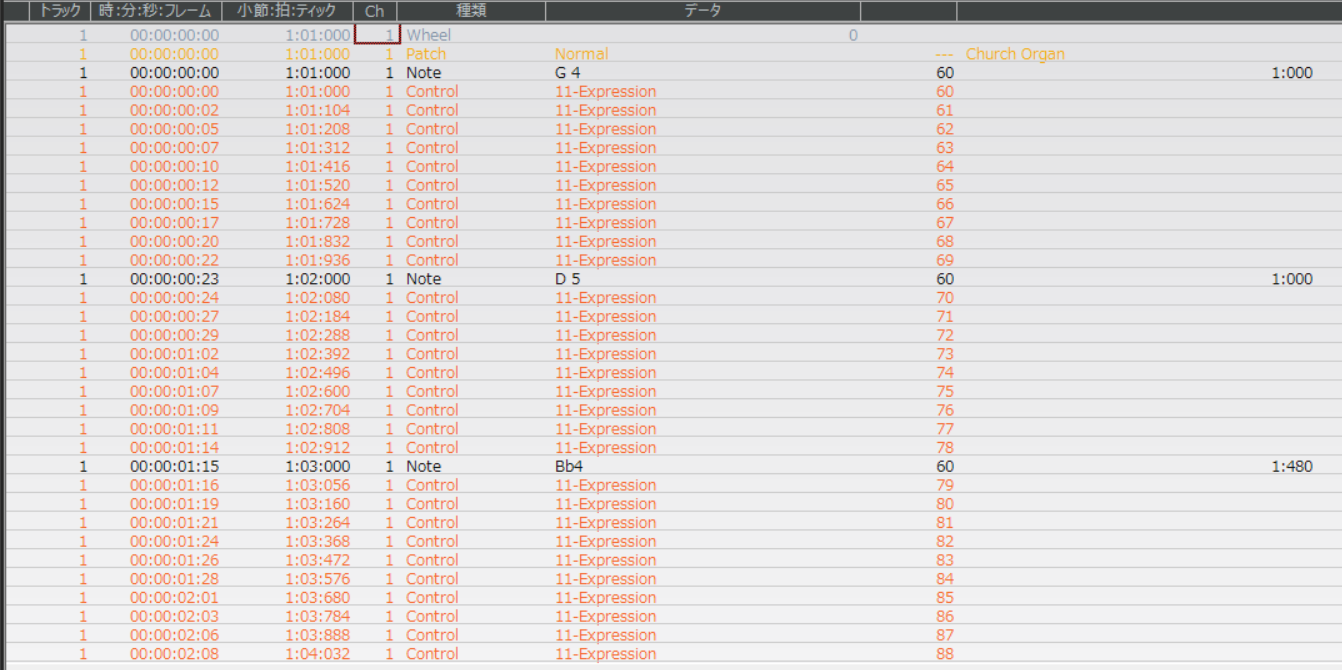
\includegraphics[width=\hsize]{fig/eventlist.png}
	%\caption{音情報のイベントリスト}
	%\label{fig:text}
%\end{figure}
\begin{figure}[tb]
	\centering
	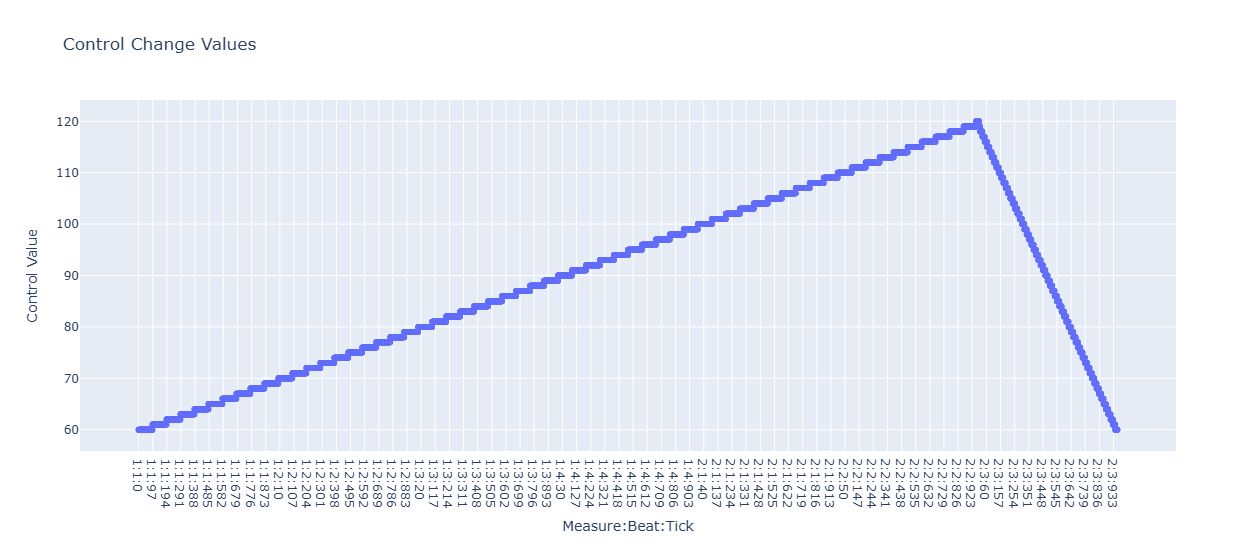
\includegraphics[width=\hsize]{fig/graph_Expression.png}
	\caption{Expression値の変化}
	\label{fig:Expression}
\end{figure}


また，フレーズを定義した際に，違和感なく強弱感を出せるように同様の間隔でExpressionを挿入している．
また，フレーズ開始〜頂点と頂点〜フレーズ終了地点のExpressionの値を計算式で表すと以下のようになる．

\begin{itemize}
	\item フレーズの開始から頂点まで：
		\begin{equation}
		E(t) = E_{\text{start}} + \left( \frac{E_{\text{peak}} - E_{\text{start}}}{t_{\text{peak}} - t_{\text{start}}} \right) (t - t_{\text{start}})
		\end{equation}


	\item 頂点からフレーズの終了まで：
		\begin{equation}
		E(t) = E_{\text{peak}} - \left( \frac{E_{\text{peak}} - E_{\text{end}}}{t_{\text{end}} - t_{\text{peak}}} \right) (t - t_{\text{peak}})
		\end{equation}
\end{itemize}

ここで，式(1)(2)の$t_{\text{peak}}$は頂点でのティック値，$E_{\text{peak}}$は頂点でのExpression値となっている．

式(1)の$t$は現在のティック数（$t\in[t_{\text{start}},t_{\text{peak}}]$)，$t_{\text{start}}$はフレーズの開始時のティック値，$E_{\text{start}}$はフレーズ開始時のExpression値である．

式(2)の$t$は現在のティック数（$t\in[t_{\text{peak}},t_{\text{end}}]$)，$t_{\text{end}}$はフレーズの終了時のティック値，$E_{\text{end}}$はフレーズ終了時のExpression値である．

フレーズ開始から頂点までの補間は，線形補間でExpression値が増加していき，頂点からフレーズ終了までの補間は，Expression値が減少していく部分となっている．これらの計算により，フレーズ全体のExpression値の変化を均等に計算することが可能である．

{\color{blue}以下追加部分
\subsubsection{フレーズの階層についての対策}
フレーズ指定の際，楽曲の旋律によっては，フレーズを複数まとめ，大きなフレーズとして扱うことがある．波形を視覚化すると，保科理論の\figref{fig:hoshina}のようになる．

例として，\figref{fig:kaiso}のようなフレーズを持った旋律を挙げる．このような場合，本システムでは，小フレーズを指定するごとに開始Expressionを自動的に前のフレーズの終了Expressionの値に設定される．値を引き継いで強弱表現を施すことで，フレーズごとに強弱の山が途切れず，大きなフレーズであるかのように強弱が反映される．

\figref{fig:kaiso-glaf}は例に挙げた数値で実装した際，Expressionの値の推移をグラフ化したものである．}
\begin{figure}[tb]
	\centering
	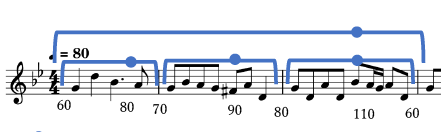
\includegraphics[width=\hsize]{fig/kaiso.png}
	\caption{階層化したフレーズ}
	\label{fig:kaiso}
\end{figure}
\begin{figure}[tb]
	\centering
	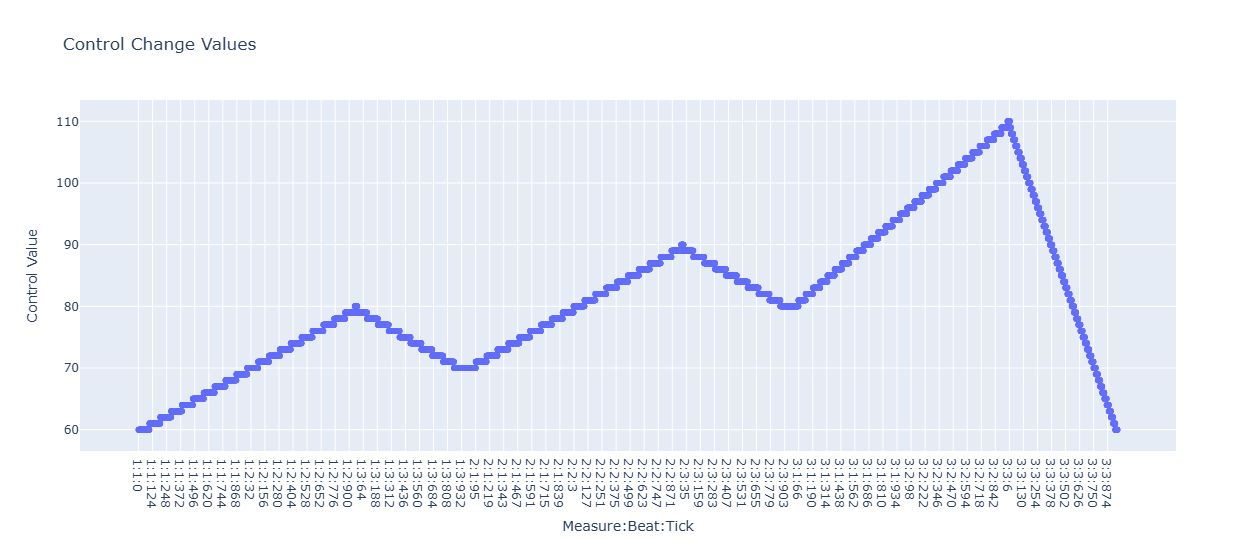
\includegraphics[width=\hsize]{fig/kaiso-graph.png}
	\caption{階層化したフレーズでのExpression値の推移}
	\label{fig:kaiso-graph}
\end{figure}


\section{実装}
本章では，構築したシステムにMIDIファイルを読み込み，強弱表現を付与したものについて記載する．
本実装に使用した楽曲は，ヨハン・ゼバスティアン・バッハ作曲の「フーガ ト短調 BWV 578」\cite{Bach}である．
選曲理由としては，テンポが遅めであり音量の変化が明確化されやすいため，この楽曲を用いて実装を行った．

また実装する音源は，単旋律の譜表で構成されたMIDIデータを作成した．原曲は鍵盤楽器のため，１段の譜表で複数旋律存在しており，強弱表現を付与した際に違いが不明瞭になると考えたからである．

楽器編成は持続音系楽器を対象としているため，オーボエ，B\Flat クラリネット，アルトクラリネット，ファゴットの４パートで作成した．

\figref{fig:9}に，CUI上での実行例と，\figref{fig:Fugue}に４パートがすべて揃う１～23小節目までの譜面を示す．
\figref{fig:oboe}と同様に，枠で囲ってあるのがフレーズ，丸で印をつけた位置をフレーズ内の頂点としている．また，頂点の丸印上部に記載されている数値は頂点でのExpression値を表している．
%\textcolor{blue}{出力した演奏音源は以下リンクから聞くことができる．https://…}

\begin{figure}[tb]
	\centering
	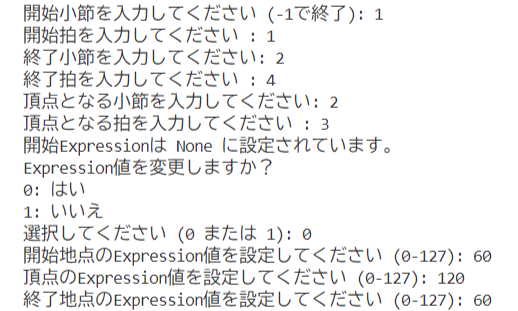
\includegraphics[width=.9\hsize]{fig/fig9-CUI.png}
	\caption{CUIシステムでの実行例}
	\label{fig:9}
\end{figure}
\begin{figure*}[tb]
	\centering
	\begin{minipage}{0.45\hsize}
		\centering
		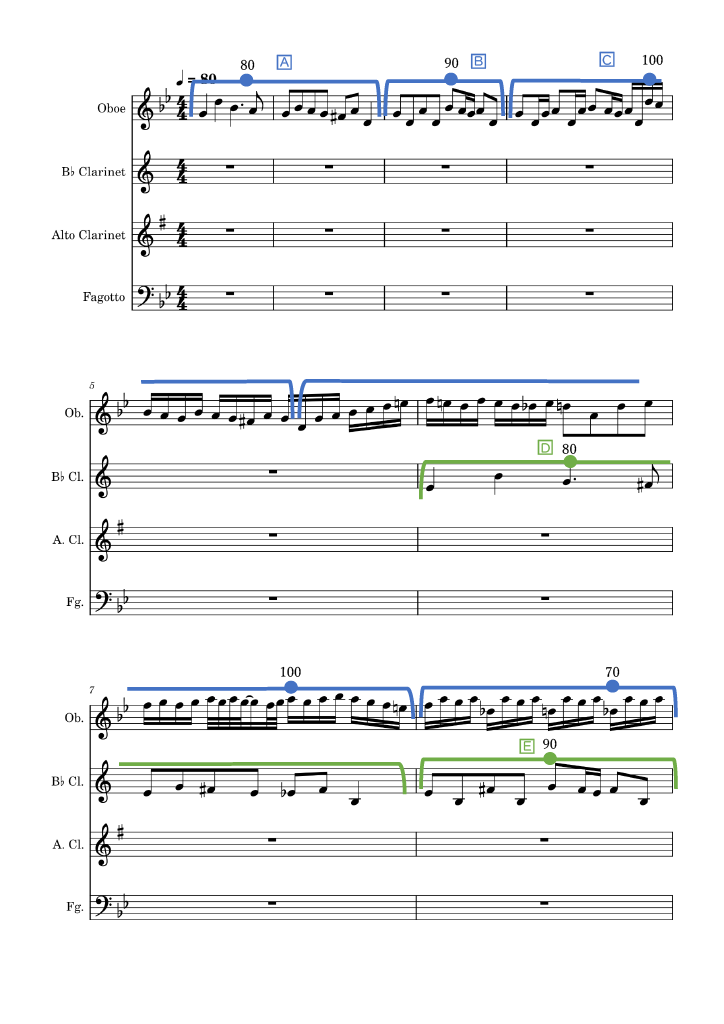
\includegraphics[width=\hsize]{fig/fig6-Fugue01.png}
		\subcaption{１～８小節}
		\label{fig:Fugue01}
	\end{minipage}
	\begin{minipage}{0.45\hsize}
		\centering
		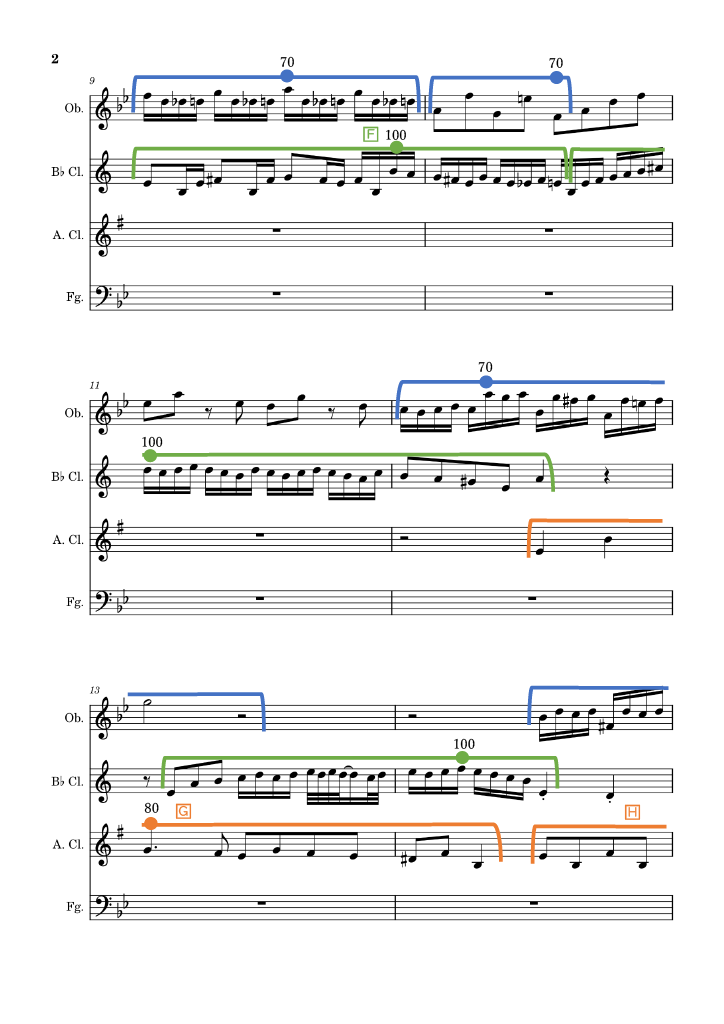
\includegraphics[width=\hsize]{fig/fig7-Fugue02.png}
		\subcaption{９～14小節}
		\label{fig:Fugue02}
	\end{minipage}
	\vspace{0.5cm}
	\begin{minipage}{0.45\hsize}
		\centering
		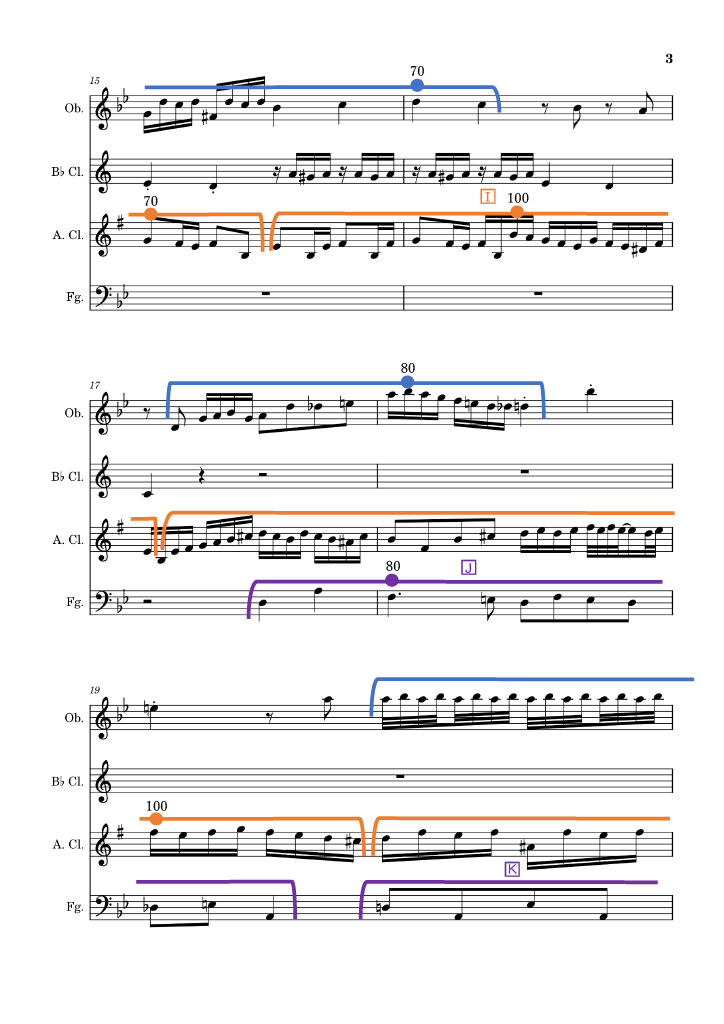
\includegraphics[width=\hsize]{fig/fig8-Fugue03.png}
		\subcaption{14～19小節}
		\label{fig:Fugue03}
	\end{minipage}
	\begin{minipage}{0.45\hsize}
		\centering
		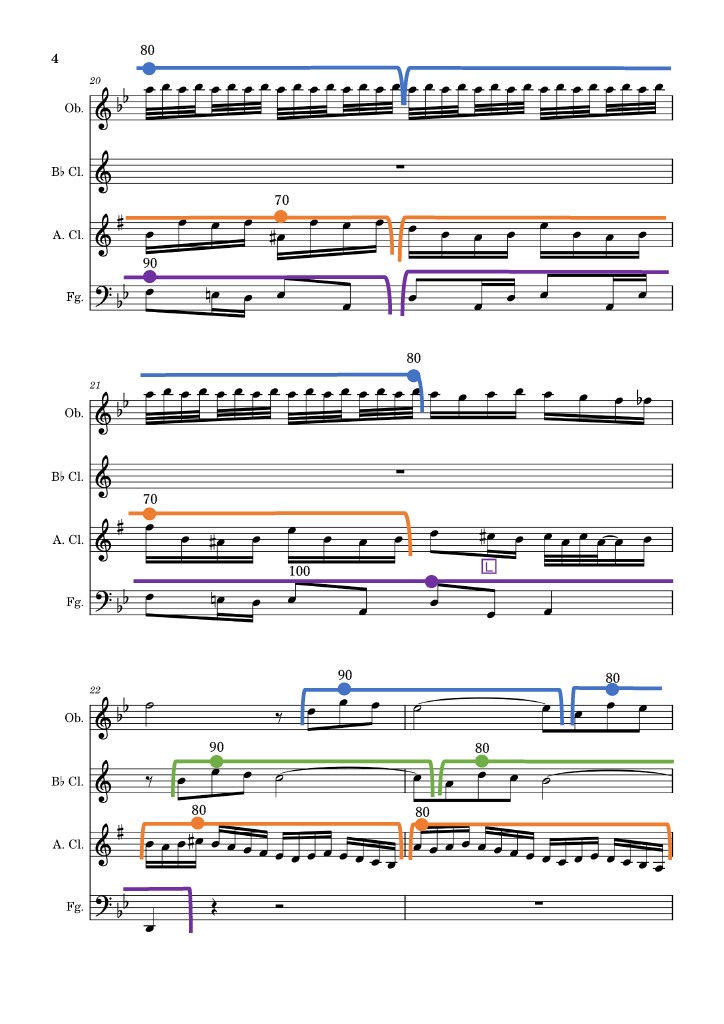
\includegraphics[width=\hsize]{fig/fig9-02-Fugue04.png}
		\subcaption{20～23小節}
		\label{fig:Fugue04}
	\end{minipage}
	\caption{「フーガ ト短調 BWV 578」に対する強弱表現}
	\label{fig:Fugue}
\end{figure*}



\subsection{track0：Oboe}
パート全体のVelocity：60

(A)フレーズ：１小節１拍～２小節4拍

・頂点：１小節3拍目

・頂点のExpression値：80


(B)フレーズ：３小節１拍～３小節４拍

・頂点：３小節３拍目

・頂点のExpression値：90


(C)フレーズ：４小節１拍～５小節３拍

・頂点：４小節4.5拍目

・頂点のExpression値：100

\subsection{track1：B\Flat Clarinet}
パート全体のVelocity：60

(D)フレーズ：６小節１拍～７小節４拍

・頂点：６小節３拍目

・頂点のExpression値：80

(E)フレーズ：８小節１拍～８小節4.5拍

・頂点：８小節３拍目

・頂点のExpression値：90


(F)フレーズ：９小節１拍～10小節３拍

・頂点：９小節4.5拍目

・頂点のExpression値：100

\subsection{track2：Alto Clarinet}
パート全体のVelocity：60

(G)フレーズ：12小節３拍～14小節２拍

・頂点：13小節１拍目

・頂点のExpression値：80


(H)フレーズ：14小節３拍～15小節３拍

・頂点：15小節１拍目

・頂点のExpression値：70


(I)フレーズ：15小節３拍～17小節１拍

・頂点：16小節2.5拍目

・頂点のExpression値：100

\subsection{track3：Fagotto}
パート全体のVelocity：60

(J)フレーズ：17小節３拍～19小節3拍

・頂点：18小節１拍目

・頂点のExpression値：80


(K)フレーズ：19小節３拍～20小節2.5拍

・頂点：20小節１拍目

・頂点のExpression値：90

(L)フレーズ：20小節３拍～22小節１拍

・頂点：21小節3拍目

・頂点のExpression値：90

\section{考察}
本システムの実装により，鍵盤楽器だけではなく，管楽器といった，音が持続する楽器に対しても音源に強弱表現の付与が可能となった．
設計から実装までの過程を通して，本システムの有用性について，見出しを分けて考察する．

\subsection{持続音楽器のための演奏表現支援}
既存研究として，管楽器演奏における演奏表現支援として， Dannenbergと堀内らのシステムを挙げる．

Dannenberg\cite{Dannenberg84a}のシステムは，リアルタイムでコンピュータが演奏者のタイミングやテンポに追従し，演奏支援を行うことに特化している．演奏者が表現の自由度をもって演奏できるのが大きな特長である．

一方，堀内らのシステムは\cite{horiuchiyasuo04}は管楽器演奏の際に生じるブレスに着目し，奏者同士の相互作用に基づいた制御を行っている．特に，ブレスが演奏に影響を及ぼすのは管楽器特有の技法である．その技術を反映させることに重きを置き，演奏者のタイミングや強弱をリアルタイムで調整するためのモデルが組み込まれている．

管楽器演奏において，強弱表現は息のコントロールによって生み出されるものであるため，鍵盤楽器等と比較して，多様な強弱表現が顕著に表れる．
また，管楽器はアンサンブルや合奏といった，複数人で演奏する機会が非常に多い．
そのため，演奏表現に関しては奏者が各々感覚で掴んでいくもの，また合奏という場においては，指導者の裁量に従いながら演奏表現を調整することが多い．

本システムでは，演奏者が意図する強弱のニュアンスを忠実に再現できる．また，楽器を使った練習でなくとも，演奏者が望む強弱感を自由に設計し，俯瞰して演奏を聴くことが実現する．
これにより，合奏といった場に挑む前に奏者自身の強弱表現を準備した状態で，演奏に反映することができる．



\subsection{楽器の特性に合わせた強弱表現の柔軟性}
本システムは，フレーズ内の強弱表現を柔軟に設定できることが特徴である．フレーズの開始地点，終了地点，頂点の設定を行うことで，フレーズ内の強弱表現を自由に設定できる．
また，フレーズ内の頂点を設定することで，強弱表現の変化を滑らかにすることが可能となる．
従来研究では，MIDIを扱うという特性上，管楽器や弦楽器などの楽器音源を用いる場合でも鍵盤楽器での強弱表現に準拠したシステムが多かった．
しかし，本システムは持続音系楽器に対しても強弱表現を付与できるため，演奏表現の幅を広げることができる．
特に，持続音楽器ならではのロングトーンの表現に関して，本システムは，音量表現を全面的にExpression値で表現することにより実現可能とした．従来研究になかった新たな視点を提供している．


実装において，特に各パートに対してフレーズの強弱表現が必要であると実感した．
既存研究では，鍵盤楽器の楽曲が前提となっている．
鍵盤楽器での演奏はソロ演奏が大半であり，1人の奏者が主旋律も副旋律も担っているため，主旋律にのみフレーズの決定が施されることが多々あった．

しかし，管楽器では旋律に対して一人のプレイヤーが演奏する．
そのため１つのパートに対して1人の奏者が存在し，それぞれが演奏する旋律に対して独立した表現を加える．そのため，各パートごとにフレーズの決定と強弱表現が重要であると考える．
この点において，パートごとの音源に詳細な強弱表現を施せるという，器楽曲の醍醐味を実装することが期待される．

\subsection{演奏シミュレータとしての課題}
一方で，「Mixtract」のメリットであった，フレーズ及びフレーズ内の頂点の推定は本システムでは行っていない．「Mixtract」では，ユーザ側にすべてのフレーズの設定を委ねられているわけではない．そのため，音楽初心者から上級者までの幅広いユーザ層に対しても，直感的に操作できるように設計されている．

しかし，本システムはフレーズ及び頂点の自動推定は行っていない．そのため，楽譜と照らし合わせながらの操作が必要であることが重要となっていること，また，楽器を演奏するようなユーザが対象者として適切だと考える．「Mixtract」と比較すると，直感的に操作することはできないため，ユーザ層は，演奏に対して理解のある中級者から上級者としている．
合奏中に手探り状態で指示を進めていくよりも，合奏に移る前の段階などでこのシステムを用いて強弱表現のシミュレーションもできるようになることが期待できる．

\section{おわりに}
本研究では，持続音系楽器の演奏表現を与える支援システムを開発した．特にロングトーンにおける強弱変化に焦点をあて，詳細な表現を加えられる柔軟な環境の構築が可能となった．
本システムの導入により，楽器演奏者が合奏の準備段階や演奏表現のシミュレーションにおいて効果的なツールとして活用できる可能性が示唆された．また，管楽器をはじめとした楽器の特性に考慮した表現が可能となり，演奏解釈や表現の幅を広げる一助となることが期待されると考えた．





%\begin{acknowledgment}
	%本稿の執筆にあたり，参考文献に挙げた方々のWebサイト，スライド，各種資料を大いに参考にさせていただいた．
	%書くならお好きに
%\end{acknowledgment}
